\section {Eksperymenty}
\subsection {Eksperyment pierwszy: pomieszczenie codziennego użytku}
Pierwszy z wykonanych eksperymentów polegał na wygenerowaniu obrazu pomieszczenia w którym pracowałem nad pisaną właśnie pracą dyplomową (salon z aneksem kuchennym).
Pomieszczenie ma XX metrów kwadratowych i znajdują się w nim elementy codziennego użytku - lodówka, zlew kuchenny, kwiaty na parapecie oraz otwór dzwiowy łączcy pomieszczenie z przedpokojem. Wymiary pokoju to XX m x XX m.\\

Pomniższy rysunek przedstawia architektoniczny rzut pomieszczenie wykonany przez mgr arch. Izabelę Jaroszek (fragment zakupionej w czasie remontu adaptacji wnętrza):
\begin{figure}[h]
    \centering
    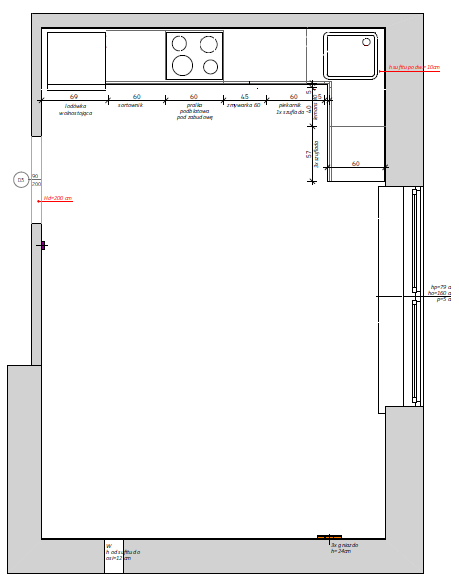
\includegraphics[scale=0.75]{experiment_1_rzut}
    \caption{Rzut architektoniczny salonu z aneksem kuchennym}
    \label{fig:experiment_1_rzut}
\end{figure}

Dla opisanego pomieszczenia wygenerowany został następujący obraz:
\begin{figure}[h]
    \centering
    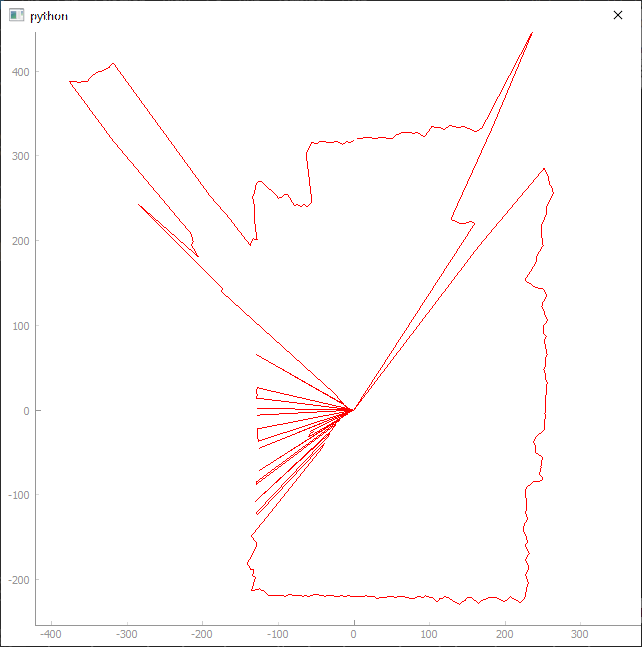
\includegraphics[scale=0.5]{experiment_1_plot}
    \caption{Wygenerowany obraz pomieszczenia - salonu z aneksem kuchennym}
    \label{fig:experiment_1_plot}
\end{figure}

W chwili generowania obrazu dalmierz znajdował się ok. 110 cm ponad powierzchnią podłogi, dzięki czemu nie znalazły się na nim stojące w pokoju umeblowanie.

\subsection {Eksperyment pierwszy: analiza wygenerowanego obrazu}

Wygenerowany obraz przedstawia dosyć wierne odwzorowanie badanego pomieszczenia. Ze względu na amatorski charakter urządzenia znalazło się w nim jednak kilka przekłamań:

\begin{enumerate}
    \item Otwór dzwiowy spowodował odczyt odległości do ściany w sąsiednim pomieszczeniu (przedpokoju) oraz kolejnym pokoju.
    \item Połyskująca powierzchnia lodówki wprodziła przekłamanie na jej frontowej powierzchni - wygenerowany jej obraz sprawia mylne wrażenie rombu. 
    \item Metalowy kran o obłym krztałcie prowadza kilka znieszkałceń - ze względu na refleksję promienia lasera.
    \item Na parapecie stoją doniczki z kwiatami co uwzględnione zostało na neregularnych kształtach wykresu
    \item Puste ściany z kąty proste odzwierciedlone zostały w dosyć dużą dokładnością.
    \item Ściana na przeciw okna została odzwierciedlola z kilkoma przekłananiami (odczyty zerowych wartości dalmierza). Powierzchnia w tym miejscu nie różni się niczym od pozostałch powierzni, zarówno użytą farbą, kolorem jak i nasłonecznieniem. Przyczyna błędnych wskazań w tym miejscu pozostaje nieznana.
    \item Wymiary pomieszczenia odzwierciedlają stan faktyczny.
\end{enumerate}
\begin{figure}[h]
    \centering
    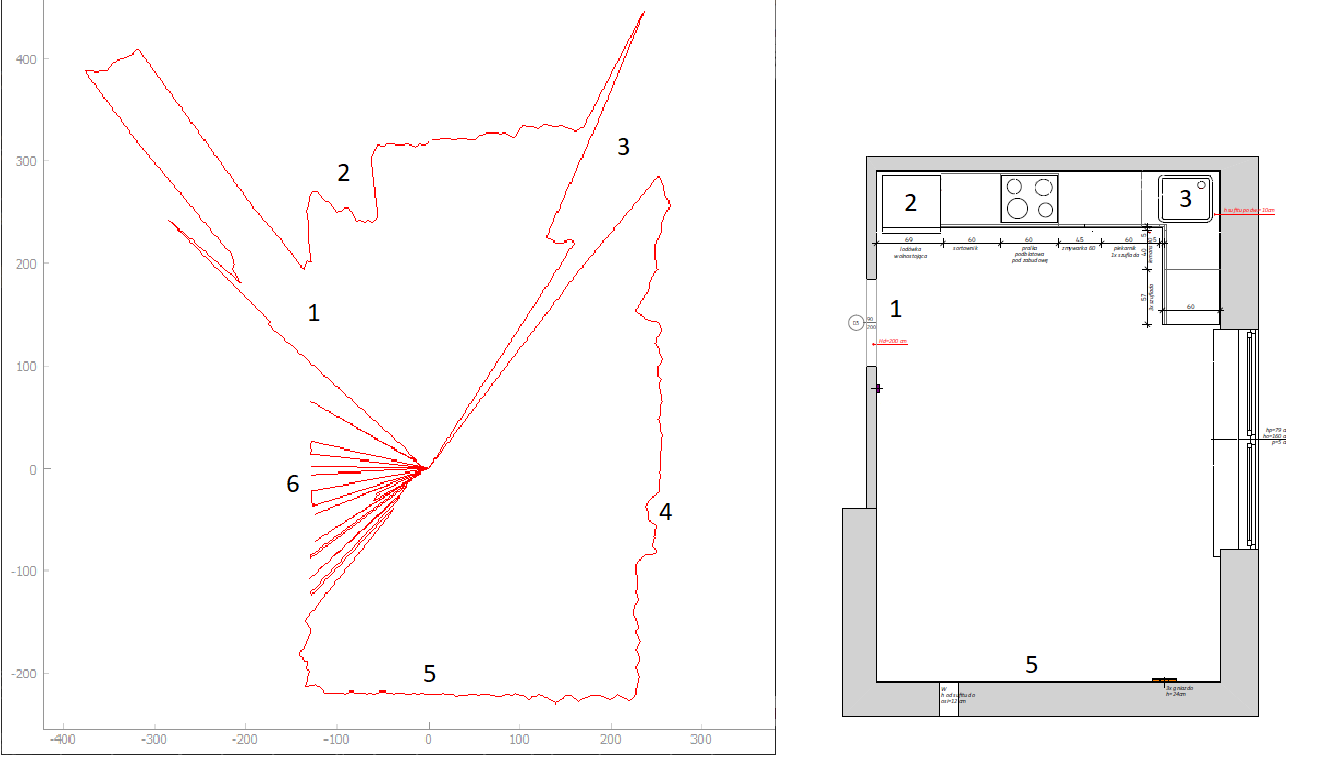
\includegraphics[scale=0.40]{experiment_1_comp}
    \caption{Porównanie obrazu z rzutem}
    \label{fig:experiment_1_comp}
\end{figure}


\newpage
\subsection {Eksperyment drugi: ocena użytej rodzielczości}

W drugim eksperymencie chciałem przekonać się o dokładności dalmierza i o tym czy zastosowana przez mnie rodzielczość (400 króków na pełen obrót) jest wystarczająca.\\

W tym celu wyłączyłem zasilanie silnika krokowego, przez co dalmierz zczytywał wciąż tę samą ogległość. Program jednak nadawał sygnał do zmiany kąta przez co przekonany był o obrocie silnika. W skutek tego otrzymaliśmy obraz okręgu (ta sama odległość dla "każdego" z kątów).

\begin{figure}[h]
    \centering
    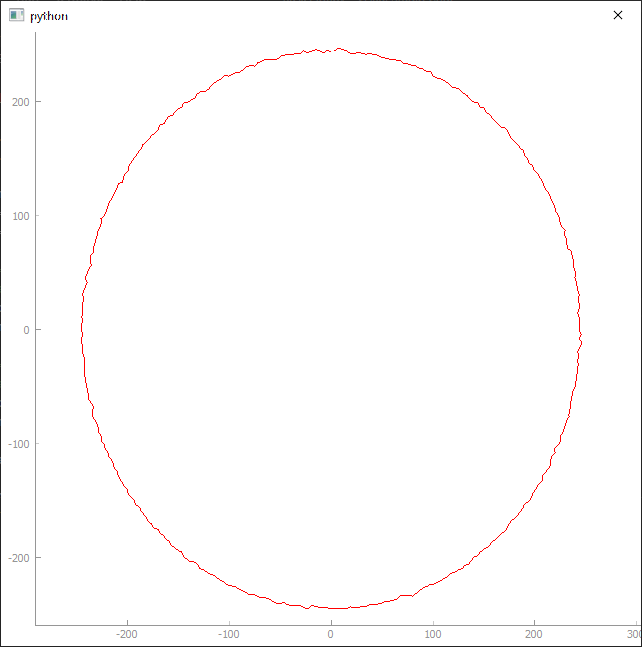
\includegraphics[scale=0.5]{experiment_2_plot}
    \caption{“Time is a flat circle” Friedrich Nietzsche}
    \label{fig:experiment_2_plot}
\end{figure}

\subsection {Eksperyment drugi: analiza wygenerowanego obrazu}
Wahania odczytów dalmierza różniły się od siebie z reguły o 1-2 cm, czasem o 3 cm. Wartość ta mieści się w podawanym w specyfikacji producenta zakresie.\\

Ilość wygenerowanych punktów (400) pozwoliła odwzorować okrąd z bardzo dużą dokładnością. Krzywizna okręgu jest gładka a jej krztałt nie jest sprawia wrażenia widocznych pixeli (prostych linii wynikających ze zbyt rzadkiej siatki punktów). Nie ma potrzeby zwiększania rozdzielczości pracy urządzenia.\\

\newpage
\subsection {Eksperyment trzeci: pomieszczenie z licznymi płaszczyznami}
Pomieszczenie do kolejnego ekperymentu wybrane zostało ze względu na duże rozmary i liczne płaszczyzmy o różnym radzaju powierzchni (firanki, ekran telewizora, okna, lodówka, połyskująca poręcz, granitowe schody).

\subsection {Eksperyment trzeci: analiza wygenerowanego obrazu}
Wygenerowany obraz zawierał liczne drobne przekłamania:

\begin{enumerate}
    \item Brak żaluzji w oknach skutkował nierównomierną powierzchnią obrazu (duże wahania mierzonej odległości)
    \item Klatka schodowa była widoczna na zarysie ale szczegóły były trudne do odczytania.
    \item Połyskująca poręcz skutkowała znacznymi przekłamaniami w odczytanej powierzchni a co za tym idzie znaczne przekłamania na tym fragmencie obrazu.
    \item Powierzchnia ekranu telewizora była silnie refleksujna co spowodowało przekłamania podobne do okiennych.
    \item Falista powierzchnia firanek została odwzorowana.
    \item Liczne zerowe odczyty. Pogarszały one obraz ale nie uniemożliwiały rozpoznania kształtu pomieszczenia.
\end{enumerate}
